\documentclass[compress]{beamer}
\usepackage{ifthen,verbatim}

\newcommand{\isnote}{}
\xdefinecolor{lightyellow}{rgb}{1.,1.,0.25}
\xdefinecolor{darkblue}{rgb}{0.1,0.1,0.7}

%% Uncomment this to get annotations
%% \def\notes{\addtocounter{page}{-1}
%%            \renewcommand{\isnote}{*}
%% 	   \beamertemplateshadingbackground{lightyellow}{white}
%%            \begin{frame}
%%            \frametitle{Notes for the previous page (page \insertpagenumber)}
%%            \itemize}
%% \def\endnotes{\enditemize
%% 	      \end{frame}
%%               \beamertemplateshadingbackground{white}{white}
%%               \renewcommand{\isnote}{}}

%% Uncomment this to not get annotations
\def\notes{\comment}
\def\endnotes{\endcomment}

\setbeamertemplate{navigation symbols}{}
\setbeamertemplate{headline}{\mbox{ } \hfill
\begin{minipage}{5.5 cm}
\vspace{-0.75 cm} \small
\end{minipage} \hfill
\begin{minipage}{4.5 cm}
\vspace{-0.75 cm} \small
\begin{flushright}
\ifthenelse{\equal{\insertpagenumber}{1}}{}{Jim Pivarski \hspace{0.2 cm} \insertpagenumber\isnote/\pageref{numpages}}
\end{flushright}
\end{minipage}\mbox{\hspace{0.2 cm}}\includegraphics[height=1 cm]{../cmslogo} \hspace{0.1 cm} \includegraphics[height=1 cm]{../tamulogo} \hspace{0.01 cm} \vspace{-1.05 cm}}

\begin{document}
\begin{frame}
\vfill
\begin{center}
\textcolor{darkblue}{\Large Prompt CRUZET-4 Alignment and AlCaRecos}

\vfill
\begin{columns}
\column{0.3\linewidth}
\begin{center}
\textcolor{darkblue}{\large Jim Pivarski}

\vspace{0.2 cm}
Alexei Safonov
\end{center}
\end{columns}

\begin{columns}
\column{0.3\linewidth}
\begin{center}
\scriptsize
{\it Texas A\&M University}
\end{center}
\end{columns}

\vfill
29 August, 2008

\end{center}
\end{frame}

%% \begin{notes}
%% \item This is the annotated version of my talk.
%% \item If you want the version that I am presenting, download the one
%% labeled ``slides'' on Indico (or just ignore these yellow pages).
%% \item The annotated version is provided for extra detail and a written
%% record of comments that I intend to make orally.
%% \item Yellow notes refer to the content on the {\it previous} page.
%% \item All other slides are identical for the two versions.
%% \end{notes}

\begin{frame}
\frametitle{Muon cosmic-ray AlCaRecos}
\textcolor{darkblue}{MuAlStandAloneCosmics}

\vspace{0.2 cm}
\begin{itemize}
\item Completed alignment of endcap disks to barrel

(while they were moving)
\end{itemize}

\vfill
\textcolor{darkblue}{MuAlGlobalCosmics, MuAlZeroFieldGlobalCosmics}

\vspace{0.2 cm}
\begin{itemize}
\item Discovered a problem with handling of tracker hits
\end{itemize}
%% \hspace{-0.83 cm} \textcolor{darkblue}{\Large Outline2}
\end{frame}

\begin{frame}
\frametitle{Alignment of endcap disks}
\small

\begin{columns}
\column{0.4\linewidth}
\begin{itemize}\setlength{\itemsep}{0.2 cm}
\item Barrel-to-endcap procedure, no tracker involved (same as CRUZETs 1--3)
\item We now build tracks in a way that is insensitive to $z$ misalignment,
  so we no longer need an approximate \mbox{pre-alignment\hspace{-0.5 cm}}
\item Compute alignment corrections (e.g.\ $z$) from each hit residual
\item Disks moved during data-taking: two validity intervals
\end{itemize}

\column{0.65\linewidth}

\begin{center}
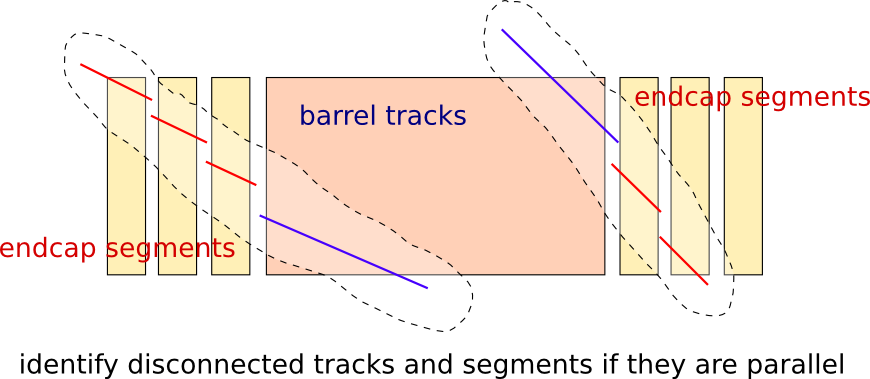
\includegraphics[width=\linewidth]{identify_if_parallel.png}
\end{center}

\vfill
\begin{center}
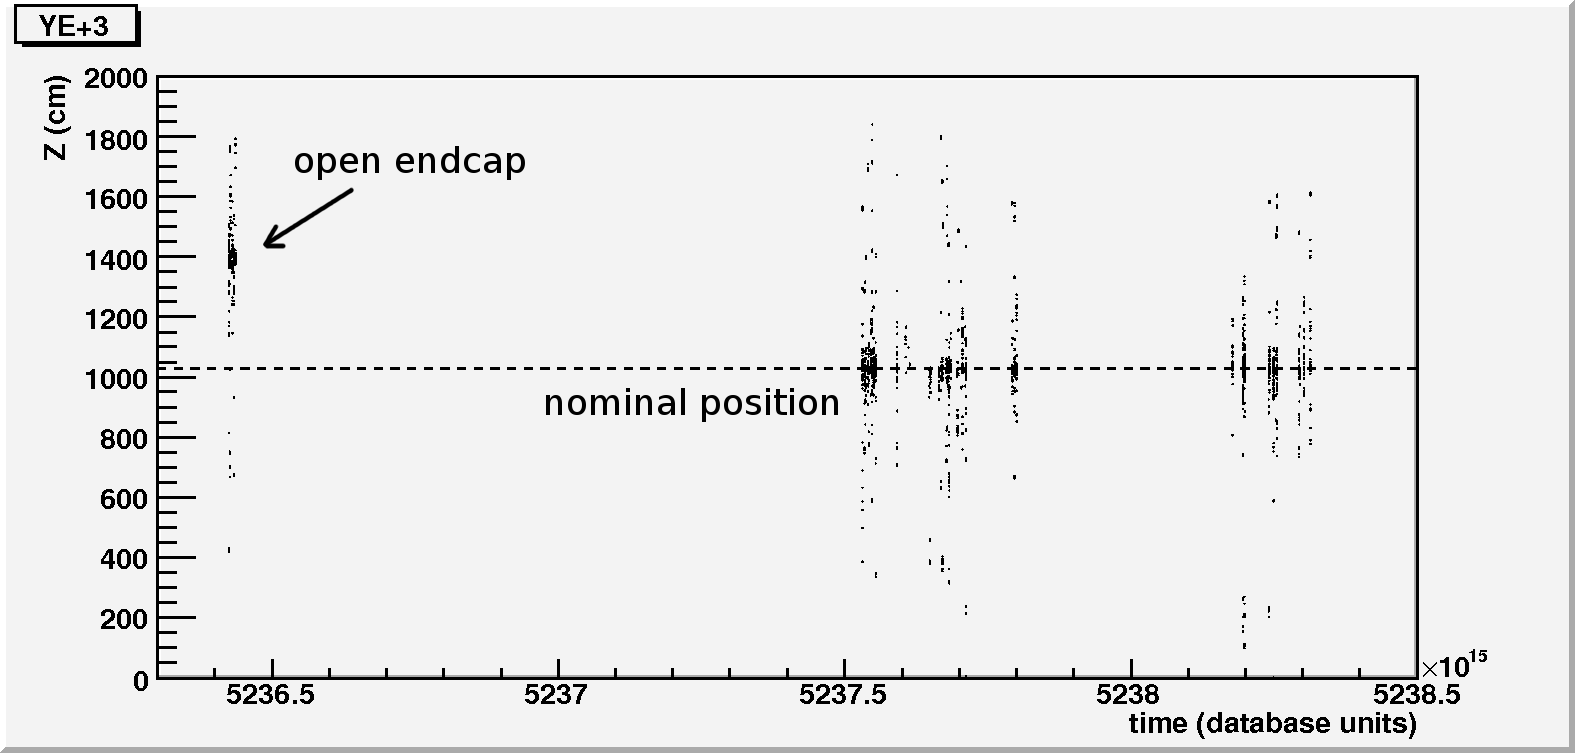
\includegraphics[width=\linewidth]{timeseries_YEp3.png}
\end{center}

\end{columns}
\end{frame}

\begin{frame}
\frametitle{Results for early period}
\small

Only one run (57795)

\vspace{0.2 cm}
\renewcommand{\arraystretch}{1.05}
\begin{tabular}{c c c c c}
 & ME$+$1 & ME$+$2 & ME$+$3 & ME$+$4 \\\hline
$\Delta z$ (cm) & $+3.1$ & $+301$ & $+301$ & $+373$ \\
& & & & \\
 & ME$-$1 & ME$-$2 & ME$-$3 & ME$-$4 \\\hline
$\Delta z$ (cm) & $-1000$ & $-1011$ & $-1011$ & $-1048$ \\
\end{tabular}

\vspace{0.6 cm}
\hspace{-0.83 cm} \textcolor{darkblue}{\Large Results for late period}

\vspace{0.2 cm}
\renewcommand{\arraystretch}{1.1}
\begin{tabular}{c c c c c c}
 & ME$+$1 & ME$+$2 & ME$+$3 & ME$+$4 & {\it (no minus-side)} \\\hline
$\Delta x$ (cm) & $0$ & $+0.3$ & $+0.3$ & $+0.5$ & \\
$\Delta y$ (cm) & $-0.5$ & $0$ & $0$ & $-0.2$ & {\it $\pm$0.2~cm} \\
$\Delta z$ (cm) & $-1.8$ & $-1.8$ & $-1.8$ & $-1.8$ & \\
\textcolor{gray}{$\Delta \phi_x$ (mrad)} & \textcolor{gray}{$+1.9$} & \textcolor{gray}{$+1.1$} & \textcolor{gray}{$+1.1$} & \textcolor{gray}{$-0.8$} & \textcolor{gray}{{\it $\pm$1~mrad (not used)}} \\
\textcolor{gray}{$\Delta \phi_y$ (mrad)} & \textcolor{gray}{$+2.0$} & \textcolor{gray}{$+1.6$} & \textcolor{gray}{$+1.6$} & \textcolor{gray}{$+1.6$} & \textcolor{gray}{{\it $\pm$1~mrad (not used)}} \\
$\Delta \phi_z$ (mrad) & $-0.3$ & $0$ & $0$ & $+0.6$ & {\it $\pm$0.25~mrad} \\
\end{tabular}

\vspace{0.2 cm}
{\it \scriptsize (ME2 = ME3 is now imposed as a constraint, used to gauge uncertainty)}
\end{frame}

\begin{frame}
\frametitle{$\Delta z$ = $-1.8$~cm? (backup slide)}
\small
\textcolor{darkblue}{Can the endcap be {\it closer} to barrel than nominal?  (a question for DPG)}

\vspace{0.3 cm}
Barrel to each station: \hfill {\it \scriptsize (nearly the same value in each)}
\begin{center}
$-1.80$~cm (ME+1), $-1.88$~cm (ME+2), $-1.85$~cm (ME+3)
\end{center}
Relative between stations: \hfill {\it \scriptsize (no gaps between stations)}
\begin{center}
$-0.32$~cm (ME+1$\to$2), $-0.03$~cm (ME+2$\to$3), $0.05$~cm (ME+3$\to$4)
\end{center}

\vspace{0.2 cm}
Aligned barrel doesn't seem to be a displaced reference because repeating endcap alignment using nominal barrel yields:
\begin{center}
$-1.3$~cm (ME+1), $-1.6$~cm (ME+2), $-2.6$~cm (ME+3)
\end{center}

\vspace{0.2 cm}
Without hit weights, $-1.8$~cm $\to$ $-1.3$~cm \hfill {\it \scriptsize (still persistently ``$-1.x$'')}

\vspace{0.3 cm}
\textcolor{darkblue}{Maybe nominal position includes a (rather large) gap?}

\vspace{0.2 cm}
Could be resolved by a conversation with the experts, but the track-based alignment results are unanimous
\end{frame}

\begin{frame}
\frametitle{Global cosmic-ray AlCaRecos}
\small

\begin{itemize}
\item Select cosmics that pass through tracker and bulid globalMuon

(two different ways, for robustness and cross-checks)
\item Purpose: for aligning muon system relative to tracker
\item Status: installed in system, produced all the data records we
  asked for, but 2\_1\_X introduced new requirements that weren't
  forseen (and weren't caught in validation)
\end{itemize}

\vfill
\textcolor{darkblue}{New in 2\_1\_X:}
\begin{itemize}
\item Tracker RecHits don't store position, must recompute from clusters
\item Muon AlCaReco selector does not store \mbox{clusters-associated-to-tracks\hspace{-1 cm}}
\begin{itemize}
\item Javier is implementing that, with help from Giovanni Petrucciani
\end{itemize}
\item Cosmic-ray AlCaRecos include all tracker clusters
\item But we don't know how to use them:

\mbox{ } \hfill globalMuon refitter module $\ne$ tracker refitter module (updated) \hfill \mbox{ }
\end{itemize}
\end{frame}

\begin{frame}
\frametitle{What we're doing about it}
\small

\begin{itemize}
\item Muon AlCaReco will store associated clusters, just like \mbox{tracker AlCaReco\hspace{-1 cm}}
\begin{itemize}
\item implementation is partly/nearly done
\item updating one C++ class corrects all muon AlCaRecos
\item will be queued as soon as it is (fully) validated
\end{itemize}

\item Two options for globalMuon refitting:
\begin{itemize}
\item teach current refitter (TracksToTrajectories) to deal with new tracker RecHits correctly
\begin{itemize}
\item configuration file changes don't seem to be sufficient
\item contacting the author
\end{itemize}

\item teach tracker refitter (TrackRefitter) to deal with muon hits
\begin{itemize}
\item would also be a C++ change
\item TrackRefitter would then provide a superset of TracksToTrajectories functionality
\end{itemize}

\end{itemize}

\item Setting up a complete muon alignment validation ``test-stand''
\begin{itemize}
\item reproduce {\it full} alignment workflow
\item RelVals will soon include AlCaReco streams
\item more manpower required, might be fulfilled within A\&M
\end{itemize}
\end{itemize}
\end{frame}

%% \section*{First section}
%% \begin{frame}
%% \begin{center}
%% \Huge \textcolor{blue}{First section}
%% \end{center}
%% \end{frame}

\begin{frame}
\frametitle{Summary and outlook}

Endcap disk alignment completed in CRUZETs 1, 2, and 4; CRUZET-3
dataset is now ready for the procedure
\begin{itemize}
\item constants sent to Luca and Pablo (both CRUZET-4 IOVs)
\end{itemize}

\vfill Discovered an inadequacy in our globalMuon AlCaRecos, but we
can fix it for the future and maybe work with it now

\vfill Tracker-to-muon alignment will need to wait for solution

\label{numpages}
\end{frame}

\end{document}
